\documentclass[xcolor={usenames,dvipsnames,svgnames}]{beamer}
\usepackage[utf8]{inputenc}
%\usepackage[usenames,dvipsnames,svgnames,table]{xcolor}
\usepackage{tikz}
\usetikzlibrary{arrows.meta}
\tikzset{>={Latex[width=2mm,length=2mm]},
  base/.style = {
    rectangle, rounded corners, draw=black,
    minimum height=1cm, text centered, font=\sffamily
  },
  process/.style = {
    base, minimum width=2.5cm, fill=orange!15,
    font=\ttfamily
  },
}

\graphicspath{{./img/},{../2021_05/img/},{../2020_03/img/}}
\DeclareGraphicsExtensions{.png,.jpg,.pdf}

\usepackage{hyperref}
\hypersetup{colorlinks,urlcolor=blue!50!black,linkcolor=red}

\usepackage{fontawesome}
\usepackage{listings}

\lstset{
  numberstyle=\tiny,
  numbersep=5pt,
  showstringspaces=true,
  %postbreak=\mbox{\textcolor{red}{$\hookrightarrow$}\space},
  basicstyle=\tiny\ttfamily,
  numbers=none,
  breaklines=true,
  extendedchars=true,
  columns=fixed,
  backgroundcolor=,
  commentstyle=\color{CadetBlue},
  stringstyle=\color{ForestGreen},
  identifierstyle=\color{Black},
}

\title{\small Máster en Sistemas Electrónicos Avanzados (MSEA)\\\Large Co-simulación y verificación funcional con\\VHDL, C/C++ y Python/m\\{\small $\{$sim$\}$}}
\author{Unai Martinez Corral\\\href{mailto:unai.martinezcorral@ehu.eus}{\faEnvelope~unai.martinezcorral@ehu.eus} ~\href{https://github.com/umarcor}{\faGithub~umarcor} ~\href{https://gitlab.com/umarcor}{\faGitlab~umarcor}}
\institute{Escuela de Ingeniería de Bilbao\\Universidad del País Vasco/Euskal Herriko Unibertsitatea (UPV/EHU)}
\date{2022/05}

\begin{document}

\frame{\titlepage}

\begin{frame}
\frametitle{Work environment}
\vfill
\begin{itemize}
  \item GHDL (LLVM or GCC backends)

  \vfill

  \item Python $>=3.6$

  \vfill

  \item Editor: Visual Studio Code (VSC), vim, emacs, Sigasi...

  \vfill

  \item GtkWave

  \vfill

  \item Language server: ghdl-ls, rust\_hdl...
\end{itemize}
\vfill
\end{frame}

\begin{frame}
\frametitle{HDL organisation in GitHub}

{\small
A joint effort from communities and companies such as GHDL, VUnit, PLC2, Symbiflow, Antmicro, Google, Chips4Makers, etc.
for gathering references, resources and pre-built/packaged solutions related to (open source) EDA tooling.
}

\vfill

\begin{minipage}{.55\linewidth}
\begin{itemize}
  \item \href{https://github.com/hdl/awesome}{hdl/awesome}
  \vfill
  \item \href{https://github.com/hdl/packages}{hdl/packages}
  \begin{itemize}
    \item \href{https://github.com/hdl/MINGW-packages}{hdl/MINGW-packages}
    \item \href{https://github.com/hdl/containers}{hdl/containers}
    \item Conda, Bazel, Termux, etc.
  \end{itemize}
  \vfill
  \item \href{https://github.com/hdl/smoke-tests}{hdl/smoke-tests}
  \vfill
  \item \href{https://github.com/hdl/constraints}{hdl/constraints}
\end{itemize}
\hfill
\end{minipage}
\begin{minipage}{.4\linewidth}
\centering
\href{https://github.com/hdl}{\includegraphics[width=3cm]{hdl_logo}}
\end{minipage}

\end{frame}


\begin{frame}[fragile]
\frametitle{Installation: on Windows (MSYS2)}
\begin{center}
\begin{minipage}{.15\linewidth}
\href{https://github.com/hdl}{\includegraphics[width=1.5cm]{hdlmsys2_logo}}
\end{minipage}
\begin{minipage}{.65\linewidth}
\href{https://hdl.github.io/MINGW-packages/\#_usage}{hdl.github.io/MINGW-packages/\#\_usage}
\end{minipage}
\end{center}

\small
\begin{enumerate}
\item Download the latest self-extracting installer or the tarball from \href{http://repo.msys2.org/distrib/x86_64/}{repo.msys2.org}
or \href{https://github.com/msys2/msys2-installer/releases}{msys2/msys2-installer}.
\item Extract/install MSYS2 and follow the guidelines in \href{https://www.msys2.org/\#installation}{msys2.org/\#installation}
for the initial sync/update.
\item On a MINGW64 shell, install the dependencies and the tools:
\end{enumerate}
\begin{lstlisting}
$ pacman -Syu --noconfirm
$ pacman -S --noconfirm p7zip git \
    mingw-w64-x86_64-yosys \
    mingw-w64-x86_64-gtkwave \
    mingw-w64-x86_64-python-pip

$ git clone --recurse-submodules https://github.com/VUnit/vunit
$ cd vunit
$ python setup.py install
\end{lstlisting}
\end{frame}

\begin{frame}
\frametitle{Installation: using containers (locally)}
\begin{center}
\begin{minipage}{.2\linewidth}
\href{https://github.com/hdl}{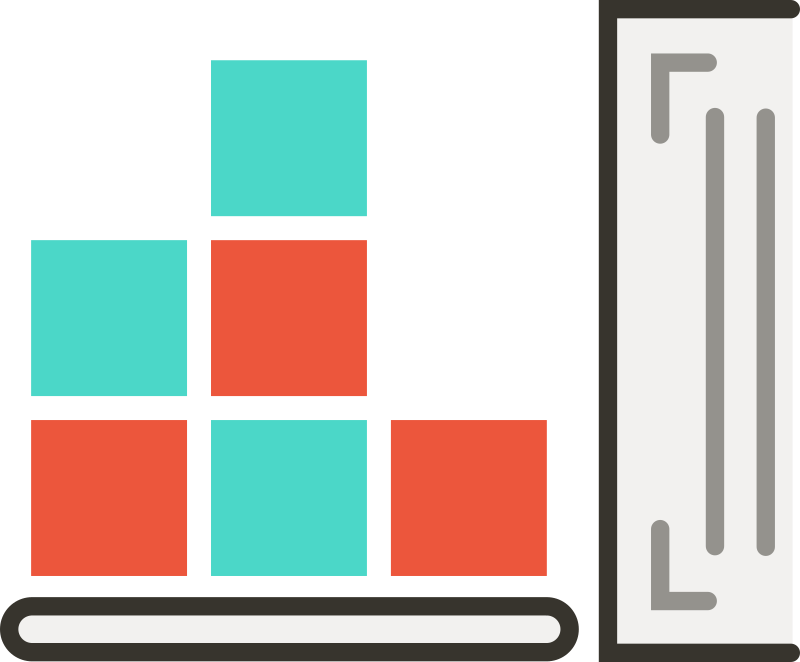
\includegraphics[width=2cm]{hdlcontainers_logo}}
\end{minipage}
\begin{minipage}{.45\linewidth}
\href{https://hdl.github.io/containers/\#_usage}{hdl.github.io/containers/\#\_usage}
\end{minipage}
\end{center}

\vfill

\begin{itemize}
\item Engine:
  \begin{itemize}
    \item Docker \href{https://www.docker.com/}{\faGlobe}
    \item Podman \href{https://podman.io/}{\faGlobe}
  \end{itemize}

\vfill

\item X server:
  \begin{itemize}
    \item x11docker \href{https://github.com/mviereck/x11docker/}{\faGithub}
    \item runx \href{https://github.com/mviereck/runx/}{\faGithub}
  \end{itemize}

\vfill

\item VSCode Remote Extensions
  \begin{itemize}
    \item Containers \href{https://marketplace.visualstudio.com/items?itemName=ms-vscode-remote.remote-containers}{\faWindows}
    \item Windows Subsystem for Linux (WSL) \href{https://marketplace.visualstudio.com/items?itemName=ms-vscode-remote.remote-wsl}{\faWindows}
  \end{itemize}
\end{itemize}
\vfill
\end{frame}

\begin{frame}
\frametitle{Installation: using online services/IDEs}
\vfill
\begin{itemize}
\item Gitpod \href{https://gitpod.io}{\faGlobe}
  \begin{itemize}
    \item \href{https://gitpod.io/\#https://github.com/umarcor/msea}{gitpod.io/\#https://github.com/umarcor/msea}
    \item \href{https://gitpod.io/\#https://github.com/cocotb/cocotb}{gitpod.io/\#https://github.com/cocotb/cocotb}
  \end{itemize}

\vfill

\item Play with Docker (PWD) \href{https://labs.play-with-docker.com/}{\faGlobe}

\vfill

\item EDA Playground \href{https://www.edaplayground.com/}{\faGlobe}

\end{itemize}
\vfill
\end{frame}

\begin{frame}
\frametitle{Exercises: introduction}
\vfill
\begin{center}
GHDL Quick Start Guide: Simulation \href{https://ghdl.github.io/ghdl/quick_start/simulation}{\faBook}
\end{center}
\vfill
\begin{itemize}
  \item Hello World
  \href{https://ghdl.github.io/ghdl/quick_start/simulation/hello}{\faBook}

  \vfill

  \item Heartbeat
  \href{https://ghdl.github.io/ghdl/quick_start/simulation/heartbeat}{\faBook}

  \vfill

  \item Full-adder
  \href{https://ghdl.github.io/ghdl/quick_start/simulation/adder}{\faBook}
\end{itemize}
\vfill
\end{frame}

\begin{frame}
\frametitle{Functional verification of an HDL design}
\centering
\includegraphics[width=\linewidth]{cosim.pdf}
\end{frame}

\begin{frame}
\frametitle{Functional verification of a non-trivial HDL design}
\centering
\includegraphics[width=\linewidth]{cosim_zoom.pdf}
\end{frame}

\begin{frame}
\frametitle{HDL simulation: VUnit}
\small
Open source unit testing framework for VHDL/SystemVerilog. It features the functionality needed to realize continuous and automated testing of your HDL code. VUnit complements traditional testing methodologies by supporting a \emph{test early and often} approach through automation.
\vfill
\begin{itemize}
  \item Supported languages: VHDL (93, 2002, 2008, 2019), Verilog, SystemVerilog
  \item Supported simulators: GHDL, Aldec Riviera-PRO/Active-HDL, Mentor Graphics ModelSim/Questa and Cadence Incisive (experimental)
  \item Requires Python $>=3.6$: Python Interface and CLI
  \item Supported on Windows, GNU/Linux and macOS.
  \item VHDL libraries: OSVVM, JSON-for-VHDL, Run, Check, Logging, Communication, Verification Components, etc.
  \item Data Types with an external API for co-simulation
\end{itemize}
\end{frame}

\begin{frame}
\frametitle{VUnit: overview}
\centering
\includegraphics[width=\linewidth]{vunit_cosim.pdf}
\end{frame}

\begin{frame}
\frametitle{Exercises: introduction}
\vfill
\begin{center}
VUnit User Guide \href{http://vunit.github.io/user_guide.html}{\faBook}
\end{center}
\vfill
\begin{itemize}
  \item Add \lstinline{run.py} to Full-adder
\end{itemize}
\vfill
\end{frame}

\begin{frame}
\frametitle{VUnit: tutorial}
\centering
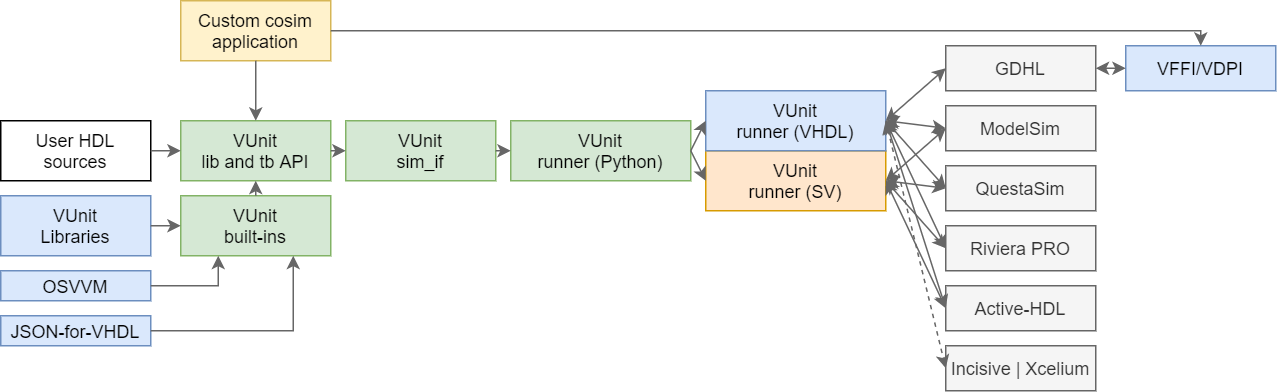
\includegraphics[width=\linewidth]{vunit.pdf}
\end{frame}

\begin{frame}
\frametitle{Exercises: libraries}
\begin{itemize}
  \item Run
  \href{http://vunit.github.io/run/user_guide.html}{\faBook}
  \href{https://github.com/VUnit/vunit/tree/master/examples/vhdl/run}{\faCode}

  \vfill

  \item Logging
  \href{http://vunit.github.io/logging/user_guide.html}{\faBook}
  \href{https://github.com/VUnit/vunit/tree/master/examples/vhdl/logging}{\faCode}

  \vfill

  \item Check
  \href{http://vunit.github.io/check/user_guide.html}{\faBook}
  \href{https://github.com/VUnit/vunit/tree/master/examples/vhdl/check}{\faCode}

  \vfill

  \item Communication
  \href{http://vunit.github.io/com/user_guide.html}{\faBook}
  \href{https://github.com/VUnit/vunit/tree/master/examples/vhdl/com/}{\faCode}

  \vfill

  \item OSVVM
  \begin{itemize}
    \item array
    \href{https://github.com/VUnit/vunit/tree/master/examples/vhdl/array}{\faCode}
  \end{itemize}

  \vfill

  \item JSON-for-VHDL
  \begin{itemize}
    \item json4vhdl
    \href{https://github.com/VUnit/vunit/tree/master/examples/vhdl/json4vhdl}{\faCode}
    \item composite\_generics
    \href{https://github.com/VUnit/vunit/tree/master/examples/vhdl/composite_generics}{\faCode}
  \end{itemize}
\end{itemize}
\vfill
\end{frame}

\begin{frame}
\frametitle{Exercises: verification components}
\begin{center}
Verification Component Library (VCL) \href{http://vunit.github.io/verification_components/user_guide.html}{\faBook}
\end{center}
\vfill
\begin{itemize}
  \item uart
  \href{https://github.com/VUnit/vunit/tree/master/examples/vhdl/uart}{\faCode}

  \vfill

  \item array\_axis\_vcs
  \href{https://github.com/VUnit/vunit/tree/master/examples/vhdl/array_axis_vcs}{\faCode}

  \vfill

  \item axi\_dma
  \href{https://github.com/VUnit/vunit/tree/master/examples/vhdl/axi_dma}{\faCode}
\end{itemize}
\vfill
\end{frame}

\begin{frame}
\frametitle{VHDL simulation: libraries/frameworks for verification}
\begin{itemize}
\item UVM: Universal Verification Methodology \href{https://en.wikipedia.org/wiki/Universal_Verification_Methodology}{\faWikipediaW}

\item OSVVM: Open Source VHDL Verification Methodolody
\href{https://osvvm.org/}{\faGlobe}
\href{https://github.com/OSVVM/OSVVM}{\faGithub}

\item UVVM: Universal VHDL Verification Methodology \href{https://bitvis.no/dev-tools/uvvm/}{\faGlobe}
\href{https://github.com/UVVM}{\faGithub}

\vfill

\item cocotb: Coroutine Co-simulation Test Bench
\href{https://github.com/cocotb/cocotb}{\faGithub}
\href{https://cocotb.rtfd.io}{\faBook}
\href{http://potential.ventures/cocotb}{\faGlobe}
\href{https://pypi.org/project/cocotb/}{\faCode}

\item VUnit: unit testing framework
\href{https://github.com/VUnit/vunit}{\faGithub}
\href{http://vunit.github.io/}{\faBook}
\href{https://pypi.org/project/vunit-hdl/}{\faCode}

\begin{itemize}
\item VUnit/cosim
\href{https://github.com/VUnit/cosim}{\faGithub}
\href{https://vunit.github.io/cosim/}{\faBook}
\end{itemize}
\end{itemize}
\end{frame}

\begin{frame}
\frametitle{Open Source Verification Bundle (OSVB)}
\centering
\Large \href{https://umarcor.github.io/osvb}{\faBook~umarcor.github.io/osvb}
\vfill
\includegraphics[width=\linewidth]{osvb}
\vfill
\includegraphics[width=2cm]{osvb_logo}
\end{frame}

\begin{frame}
\frametitle{OSVB: pyCAPI}
\centering
\vfill
\includegraphics[width=\linewidth]{pyCAPI}
\vfill
\Large \href{https://umarcor.github.io/osvb/apis/core.html}{\faBook~umarcor.github.io/osvb/apis/core}
\vfill
\end{frame}

\begin{frame}
\frametitle{OSVB: Open Source Verification Report (OSVR)}
\centering
\hspace*{1cm}
\includegraphics[width=.75\linewidth]{osvr}
\vfill
\Large \href{https://umarcor.github.io/osvb/apis/logging.html}{\faBook~umarcor.github.io/osvb/apis/logging}
\vfill
\end{frame}

\end{document}
